\documentclass{report}
\usepackage[utf8]{inputenc}
\usepackage[italian]{babel}
\usepackage[linktoc=all]{hyperref}
\usepackage{graphicx}
\usepackage{mathtools}
\usepackage{float}
\graphicspath{ {./images/} }
\hypersetup{
	colorlinks,
	citecolor=black,
	filecolor=black,
	linkcolor=black,
	urlcolor=black
}
\usepackage[a4paper,includeheadfoot,margin=2.54cm]{geometry}
\usepackage{fancyhdr}
\newcommand\hr{\par\vspace{-.5\ht\strutbox}\noindent\hrulefill\par}
\usepackage{enumitem}


\begin{document}
	
	\author{Davide Parpinello}
	\title{%
			\begin{Large}
				Appunti di\\
			\end{Large}
		Reti (F. Granelli)}
	\date{Aprile 2020}
	\maketitle
	
	\tableofcontents
	\renewcommand{\chaptermark}[1]{%
		\markboth{#1}{}}
	\addtocontents{toc}{\protect\hypertarget{toc}{}}
	\pagestyle{fancy}
	\fancyhf{}
	\rhead{\hyperlink{toc}{Reti}}
	\lhead{\leftmark}
	\rfoot{\thepage}
	
	\chapter{Roadmap}
	\section{Internet}
	
	Internet è costituito da milioni di dispositivi, chiamati \textbf{sistemi terminali}, collegati tra loro da collegamenti in rame, fibre ottiche, oppure via radio come onde elettromagnetiche o satelliti.
	\medskip\\
	La frequenza di trasmissione in internet è data dall'ampiezza di banda disponibile.
	\medskip\\Sulla rete internet inoltre sono presenti particolari host, denominati \textbf{router}, che si occupano di instradare i pacchetti verso la loro destinazione finale.
	\medskip\\Nello scambio di messaggi tra host vengono implementati dei \textbf{protocolli}, che ne definiscono formato e ordine d'invio, così come le azioni intraprese in fase di trasmissione e/o ricezione di un messaggio o un altro evento.
	\medskip\\Internet è un'infrastruttura di comunicazione per applicazione distribuita, viene anche chiamato "rete delle reti" ed è organizzato in modo gerarchico.
	\section{Ai confini della rete}
	Sul bordo della rete internet troviamo applicazioni e sistemi terminali, raggruppati tra loro e connessi tra di loro mediante collegamenti cablati e wireless.
	\medskip\\I sistemi terminali (o host) fanno girare diversi programmi applicativi e possono essere organizzati con architettura client/server oppure P2P.
	\medskip\\L'accesso a internet può avvenire mediante diversi modi:
	\begin{itemize}
		\item \textbf{Accesso residenziale:} viene utilizzato un modem dial-up o DSL.
		\item \textbf{Accesso aziendale:} una LAN collega i sistemi terminali di aziende e università all'\textbf{edge router}, i sistemi terminali sono collegati tra loro mediante uno switch ethernet.
		\item \textbf{Accesso wireless:} i terminali vengono collegati mediante \textbf{access point}.
		\item \textbf{Reti domestiche:} sono costituite da un modem DSL o via cavo, un router/firewall/NAT, switch ethernet e accesso wireless. Spesso queste funzioni vengono raggruppate in un unico dispositivo (modem/router).
	\end{itemize}
	\section{Il nucleo della rete}
	Al centro della rete si trovano invece router interconnessi tra loro, che creano quindi una rete delle reti.
	\medskip\\I dati nel nucleo della rete vengono trasferiti con due modalità differenti:
	\begin{itemize}
		\item \textbf{Commutazione di circuito:} è presente un circuito dedicato per l'intera durata della sessione
		\item \textbf{Commutazione di pacchetto:} i messaggi di una sessione utilizzano le risorse su richiesta, di conseguenza potrebbero dover attendere per accedere a un collegamento.
	\end{itemize}
	\subsection{Esempio di commutazione di circuito}
	Consideriamo un file L di 640.000 bit, un bitrate totale C da 1.536 Mbps, TDM con 24 slot/s, 500ms per stabilire la connessione.
	\medskip\\ Trovo inizialmente la capacità di un singolo slot:\[C_{1 slot} = \frac{C}{24} = 0.064 Mbps = 64 Kbps\]
	Successivamente calcolo il tempo necessario alla trasmissione:\[T_{tx} = \frac{L}{C_{1 slot}} = 10s\]
	Infine, calcolo il tempo totale:\[T_{tot}=500ms+10s=10,5s\]
	\subsection{Esempio di commutazione di circuito}
	I secondi necessari per trasmettere un pacchetto in uscita su un collegamento da R bps sono dati da L/R, mentre il ritardo 3L/R
	\subsection{Confronto fra commutazione di pacchetto e di circuito}
	La commutazione di pacchetto consente un utilizzo della rete da parte di maggiori utenti, ed è ottima per i dati a raffica.\medskip\\ Dal lato negativo, presenta un'eccessiva congestione, causando ritardi e perdite di pacchetti. Sono quindi necessari protocolli per il trasferimento affidabile e per il controllo della congestione.
	\subsection{Struttura gerarchica}
	La rete internet ha una struttura fondamentalmente gerarchica:
	\begin{itemize}
		\item Al centro sono presenti \textbf{ISP di livello 1}, che offrono una copertura nazionale e/o internazionale
		\begin{itemize}
			\item Comunicano tra loro come fossero pari
		\end{itemize}
		\item \textbf{ISP di livello 2:} ISP più piccoli, copertura nazionale/distrettuale.
		\begin{itemize}
			\item Si può connettere solo ad alcuni ISP di livello 1 e ad altri di livello 2
			\item Paga l'ISP di livello 1 che gli fornisce la connettività per il resto della rete
		\end{itemize}
		\item \textbf{ISP di livello 3 e ISP locali (di accesso):}
		\begin{itemize} 
			\item sono le reti "ultimo salto", le più vicine agli host
			\item Sono clienti degli ISP di livello superiore che li collegano all'intera internet.
		\end{itemize}
	\end{itemize}
	Un pacchetto attraversa un sacco di reti, dal livello più basso fino al principale e poi nuovamente a scendere.
	\section{Ritardi, perdite e throughput nelle reti a comunicazione di pacchetto}
	Nella rete si verificano dei ritardi quando il tasso di arrivo dei pacchetti eccede la capacità di evaderli, con la conseguenza che vengono accodati nei buffer del router in attesa del proprio turno. Se non ci sono buffer liberi i pacchetti vengono scartati e ritrasmetti dal nodo precedente o, in alcuni casi, non venire proprio ritrasmessi.
	\medskip\\ Quattro cause di ritardo dei pacchetti sono le seguenti:
	\begin{enumerate}
		\item Ritardo di elaborazione sul nodo
		\begin{itemize}
			\item Controllo errori sui bit
			\item Determinazione del canale di uscita
		\end{itemize}
		\item Ritardo di accodamento
		\begin{itemize}
			\item Attesa di trasmissione
			\item Livello di congestione del router
		\end{itemize}
		\item Ritardo di trasmissione (L/R)
		\begin{itemize}
			\item R = frequenza di trasmissione del collegamento
			\item L = lunghezza del pacchetto
		\end{itemize}
		\item Ritardo di propagazione (d/s)
		\begin{itemize}
			\item d = lunghezza dl collegamento fisico 
			\item s = velocità di propagazione del collegamento (\textasciitilde \(2 \cdot 10^8\) m/s)
		\end{itemize}
	\end{enumerate}
	\begin{center}
		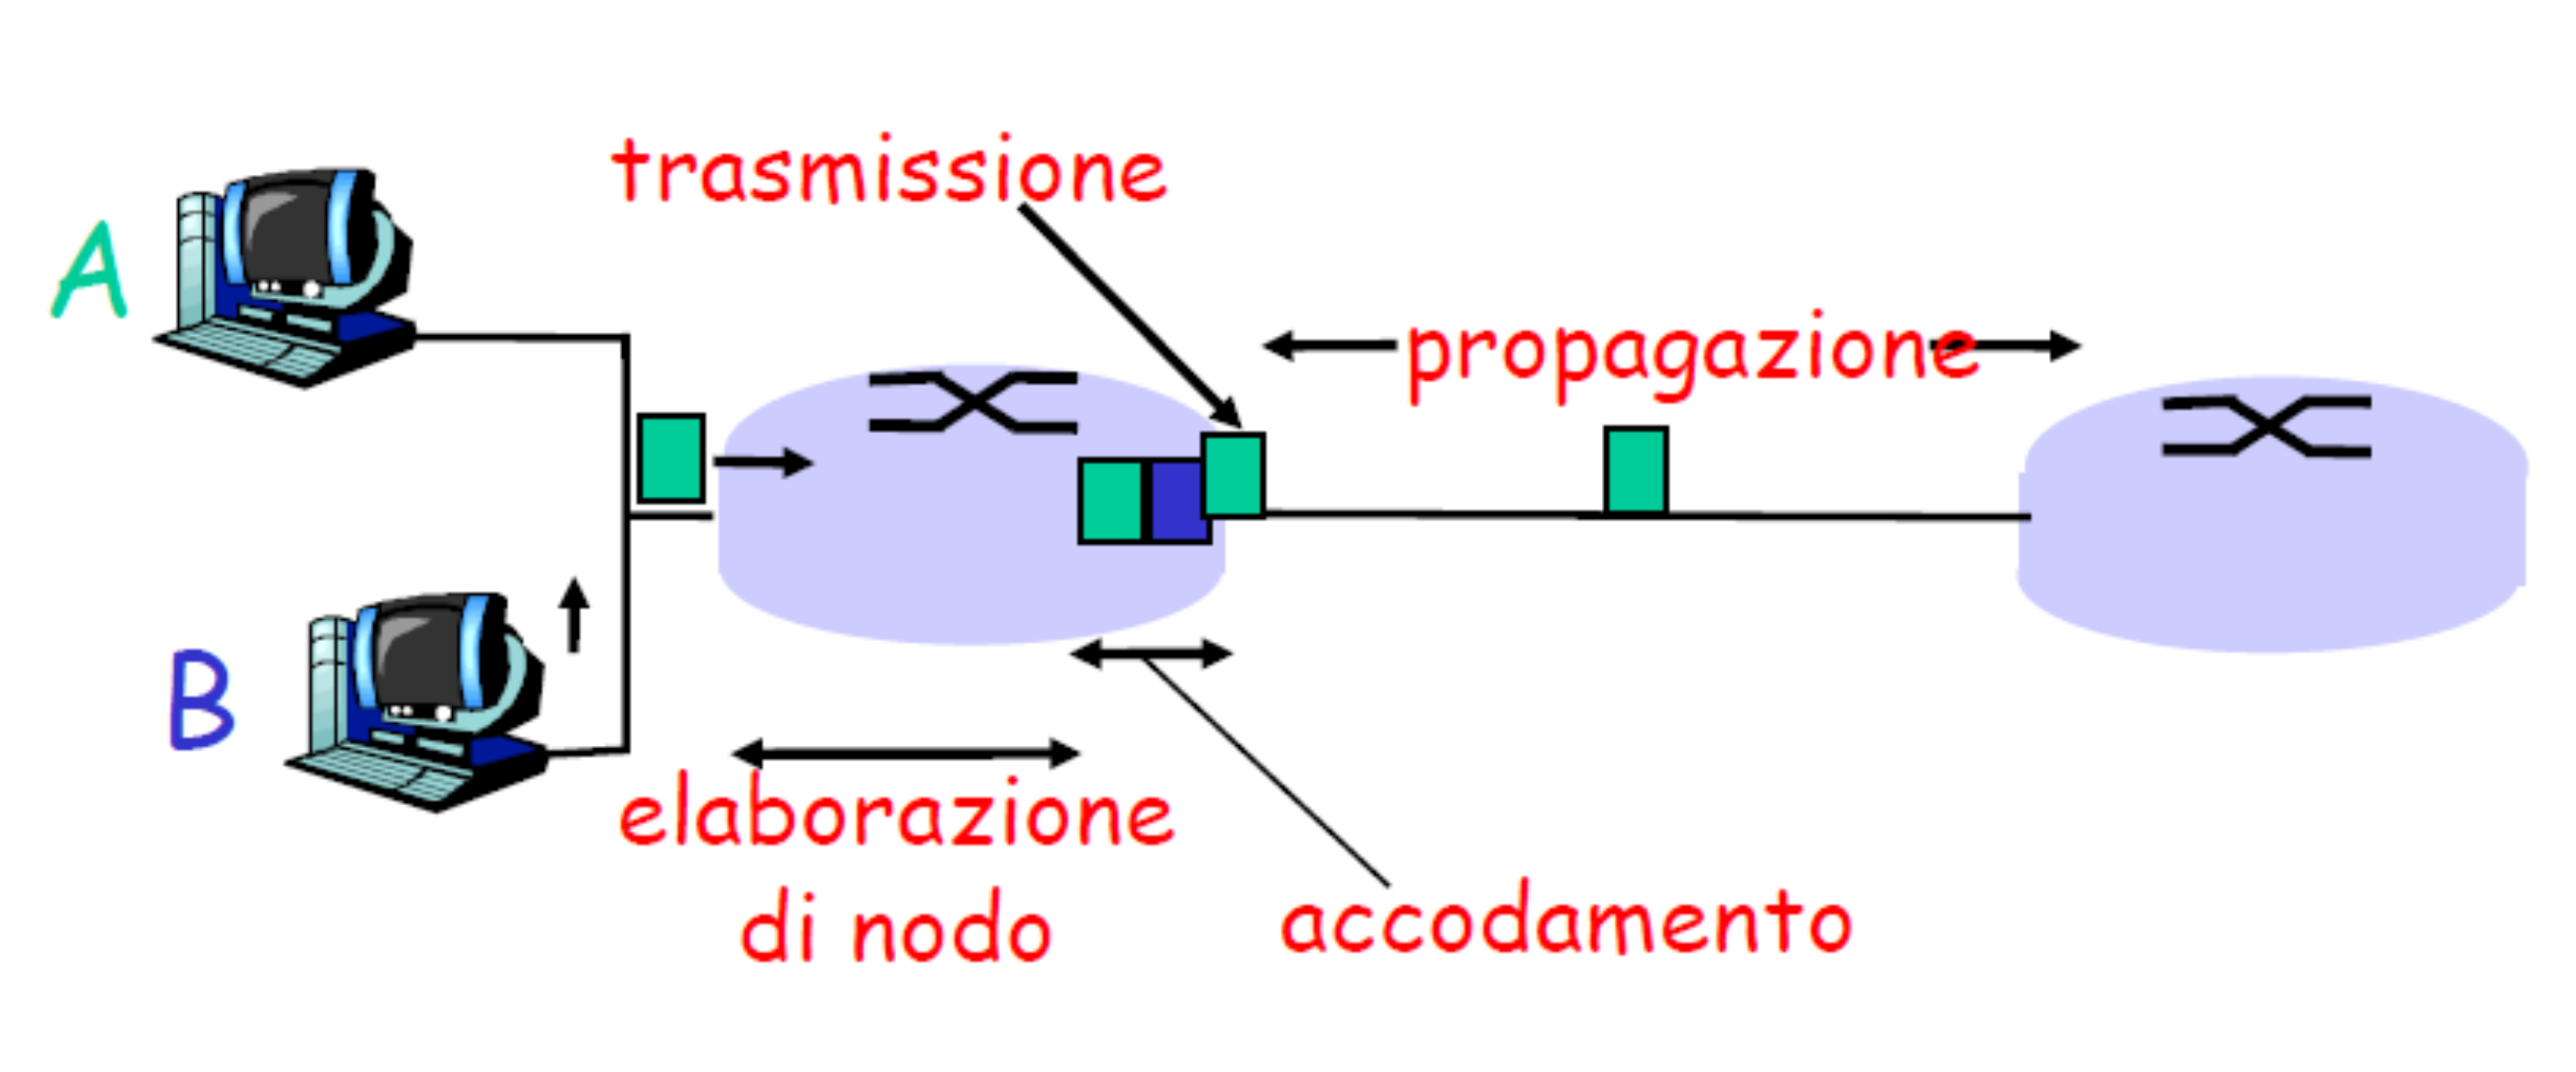
\includegraphics[width=0.7\linewidth]{ritardi.png}
	\end{center}
	\subsection{Ritardo di un nodo}
	Il ritardo di un nodo è dato dalla seguente formula:
	\begin{equation}
		d_{nodal} = d_{proc}+d_{queue}+d_{trans}+d_{prop}
	\end{equation}
	dove:
	\begin{itemize}
		\item d\textsubscript{proc} = ritardo di elaborazione (processing delay)
		\subitem- in genere di pochi microsecondi, o anche meno
		\item d\textsubscript{queue} = ritardo di accodamento
		\subitem- dipende dalla congestione
		\item d\textsubscript{trans} = ritardo di trasmissione (transmission delay)
		\subitem- significativo sui collegamenti a bassa velocità
		\item d\textsubscript{prop} = ritardo di propagazione (propagation delay)
		\subitem- da pochi microsecondi a centinaia di millisecondi
	\end{itemize}
	\subsubsection{Ritardo di accodamento}
	\begin{itemize}
		\item R = frequenza di trasmissione (bps)
		\item L = lunghezza del pacchetto (bit)
		\item a = tasso medio di arrivo dei pacchetti
	\end{itemize}
	
	Se calcoliamo La/R otteniamo l'intensità di traffico:
	\begin{itemize}
		\item Vicino a 0: poco ritardo
		\item Minore o uguale a 1: traffico consistente
		\item Maggiore di 1: più lavoro in arrivo di quanto possa essere effettivamente svolto, ritardo medio infinito.
	\end{itemize}
	Il \textbf{throughput} viene calcolato come la frequenza (bit/unità di tempo) alla quale i bit sono trasferiti tra mittente e ricevente. Può essere istantaneo o medio (in un periodo più lungo).
	\medskip\\In internet si considera anche il \textbf{collo di bottiglia}, ovvero un collegamento su un percorso punto-punto che vincola un throughput end to end.
	\section{Livelli di protocollo e i loro modelli di servizio}
	Si considerano principalmente 5 livelli di protocollo:
	\begin{enumerate}
		\item \textbf{Applicazione:} di supporto alle applicazioni di rete
		\item \textbf{Trasporto:} trasferimento dei messaggi del livello applicazione tra modulo client e server, connessione tra processi applicativi
		\item \textbf{Rete:} instradamento dei datagram dall'origine al destinatario
		\item \textbf{Link \textit{(collegamento)}:} instradamento dei datagram attraverso una serie di commutatori di pacchetto
		\item \textbf{Fisico:} trasferimento dei singoli bit
	\end{enumerate}
	\section{Reti sotto attacco: la sicurezza}
	I malintenzionati installano malware negli host attraverso internet. Il malware può raggiungere gli host attraverso virus, worm o cavalli di Troia. Un malware di spionaggio può registrare quanto viene digitato, i siti visitati e informazioni di upload. Gli host infettati possono diventare botnet e essere usati per lo spamming e attacchi DDoS. Un malware è spesso auto-replicante e da un host attaccato può passare ad altri host.
	\paragraph{Analisi di pacchetti} Chiamato anche packet sniffing, quando un'interfaccia di rete legge/registra tutti i pacchetti che la attraversano.
	\paragraph{IP spoofing} Invio di pacchetti con un indirizzo sorgente falso.
	\paragraph{Record-and-playback} Vengono "sniffati" dati sensibili per utilizzarli in un secondo momento.
	\chapter{Il livello Applicazione}
	\section{Principi delle applicazioni di rete}
	Le applicazioni di rete sono costruite con diverse architetture
	\begin{itemize}
		\item Client-Server
		\begin{itemize}
			\item L'host (o client) interagisce direttamente con il server
			\item Più client ci sono più il servizio diminuisce
		\end{itemize}
		\item Peer-to-Peer (P2P)
		\begin{itemize}
			\item Non c'è un server sempre attivo
			\item Coppie arbitrarie di host comunicano direttamente fra di loro
			\item Facilmente scalabile ma difficile da gestire
		\end{itemize}
		\item Architetture ibride
		\begin{itemize}
			\item Skype, messaggistica istantanea
			\item Connessione client-client, utilizzo del server per la ricerca dell'indirizzo della parte remota
		\end{itemize}
		\item Cloud computing
		\begin{itemize}
			\item Un insieme di tecnologie che permettono sia di archiviare dati che elaborarli tramite l'utilizzo di risorse distribuite e virtualizzate in rete
			\item Creazione di copie di sicurezza preventive in modo automatico trasferendo tutta l'operatività online
			\item Dati memorizzati in server farm
			\item Sempre client-server ma basata sulla virtualizzazione
		\end{itemize}
	\end{itemize}
	Un processo è un programma in esecuzione su un host. All'interno dell'host due processi comunicano utilizzando schemi di interprocesso, mentre su host differenti comunicano attraverso lo scambio di messaggi.
	\begin{itemize}
		\item \textbf{Processo client:} processo che dà inizio alla comunicazione
		\item \textbf{Processo server:} processo che attende di essere contattato
	\end{itemize}
	Un processo invia/riceve messaggi mediante la sua socket. La socket è analoga ad una porta mediante la quale un processo che vuole inviare un messaggio lo fa uscire. Questo presuppone l’esistenza di un’infrastruttura esterna che trasporterà il messaggio attraverso la rete fino alla porta del processo di destinazione.
	\medskip\\ Per il trasporto internet vengono utilizzati i servizi dei protocolli TCP e UDP.
	\subsubsection{Servizio TCP}
	\begin{itemize}
		\item \textcolor{red}{Orientato alla connessione:} è richiesto un setup fra i processi client e server
		\item \textcolor{red}{Trasporto affidabile} fra i processi d'invio e ricezione
		\item \textcolor{red}{Controllo di flusso:} il mittente non vuole sovraccaricare il destinatario
		\item \textcolor{red}{Controllo della congestione:} "strozza" il processo d'invio quando la rete è sovraccaricata
		\item \textbf{Non offre} temporizzazione, garanzie sull'ampiezza di banda minima, sicurezza
		\item \textbf{Più affidabile ma si paga con ritardi di trasferimento}
	\end{itemize}
	\subsubsection{Servizio UDP}
	\begin{itemize}
		\item Trasferimento dati inaffidabile fra processi d'invio e ricezione
		\item \textbf{Non offre} setup della connessione, affidabilità, controllo di flusso, controllo della congestione, temporizzazione né ampiezza di banda minima e sicurezza
		\item \textcolor{red}{Mandare i dati il più velocemente possibile ma senza completa affidabilità}, usato per gaming online e VoIP
	\end{itemize}
	\section{Web e HTTP}
	L'HTTP, o HyperText Transfer Protocol, è un protocollo a livello applicazione per il web, che considera un client che richiede, riceve e visualizza gli oggetti del Web e un server, che invia gli oggetti in risposta ad una richiesta.
	\medskip\\Viene utilizzato TCP nel seguente modo:
	\begin{itemize}
		\item Il client inizializza la connessione TCP con il server (crea una socket) tipicamente sulla porta 80
		\item Il server accetta la connessione TCP dal client
		\item Avviene lo scambio di messaggi HTTP tra browser e server web
		\item Chiusura della connessione TCP
	\end{itemize}
	HTTP è un protocollo \textit{stateless} (senza stato), cioè il server non mantiene informazioni sulle richieste fatte dal client.
	\medskip\\Le connessioni HTTP possono essere non persistenti o persistenti.
	\paragraph{RTT} Round trip time, tempo impiegato da un piccolo pacchetto per andare dal client al server e ritornare al client.
	\subsection{Connessioni non persistenti}
	Viene trasferito un solo oggetto su una singola connessione TCP. Il tempo di risposta è dato da:
	\begin{itemize}
		\item Un RTT per inizializzare la connessione TCP
		\item Un RTT per inviare la richiesta HTTP e i primi byte
		\item Il tempo necessario alla trasmissione del file
	\end{itemize}
	Quindi totale = 2 RTT + tempo di trasmissione. Le connessioni non persistenti presentano alcuni svantaggi:
	\begin{itemize}
		\item Richiedono 2RTT per ogni oggetto
		\item Overhead dell'OS per ogni connessione TCP
		\item I browser aprono spesso connessioni TCP parallele per caricare gli oggetti referenziati
	\end{itemize}
	\subsection{Connessioni persistenti}
	Il server lascia la connessione TCP aperta dopo l'invio di una risposta, i successivi messaggi tra gli stessi client/server vengono trasmessi sulla connessione aperta, il client invia le richieste non appena incontra un oggetto referenziato, un solo RTT per tutti gli oggetti referenziati.
	\subsection{Messaggi HTTP}
	I messaggi HTTP possono essere di richiesta o di risposta.
	\subsubsection{Richiesta HTTP}
	\begin{verbatim}
		GET /somedir/page.html HTTP/1.1
		Host: www.someschool.edu
		User-agent: Mozilla/4.0
		Connection: close Accept-language:fr
	\end{verbatim}
	\subsubsection{Risposta HTTP}
	\begin{verbatim}
		HTTP/1.1 200 OK
		Connection close
		Date: Thu, 06 Aug 1998 12:00:15 GMT
		Server: Apache/1.3.0 (Unix)
		Last-Modified: Mon, 22 Jun 1998 ...
		Content-Length: 6821
		Content-Type: text/html
	\end{verbatim}
	\subsection{Cookies}
	\begin{center}
		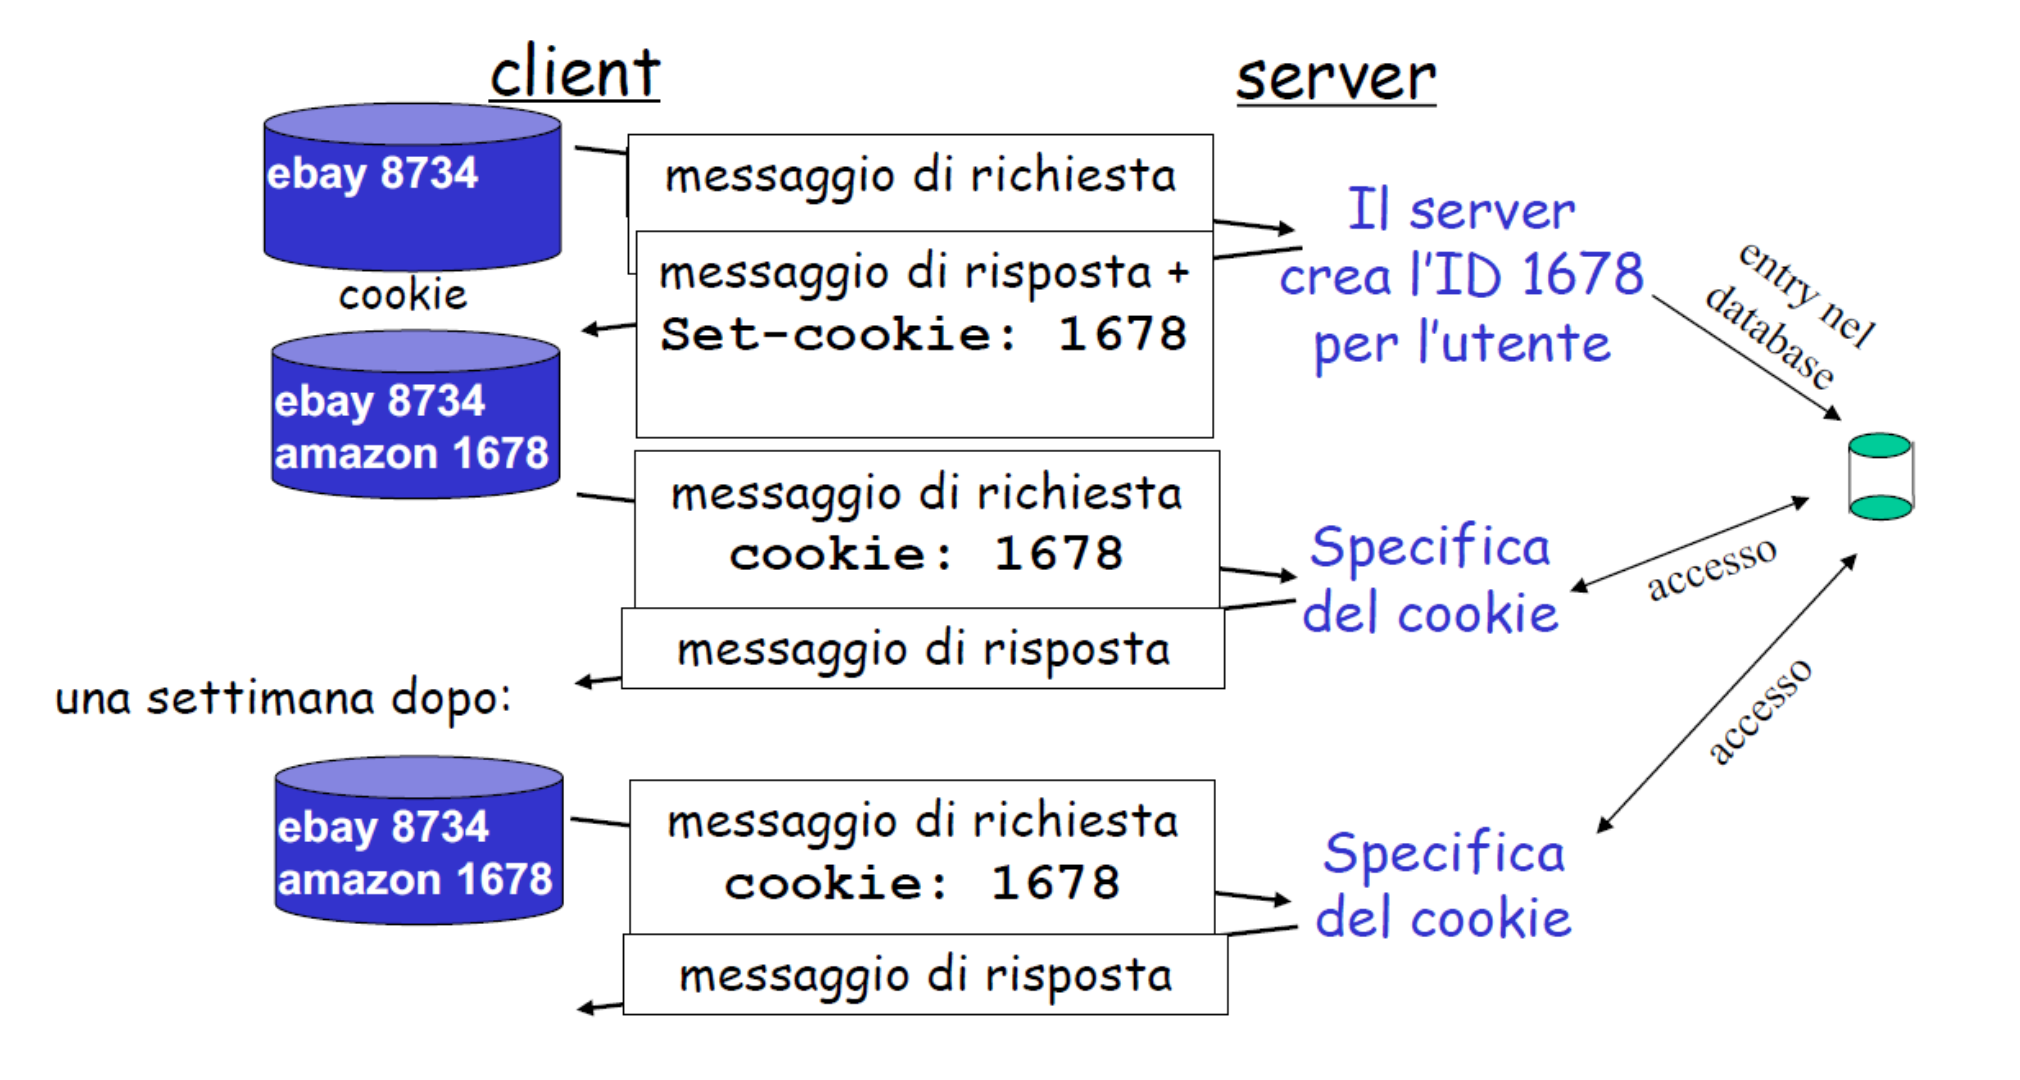
\includegraphics[width=0.7\linewidth]{cookies.png}
	\end{center}
	I cookies possono essere utilizzati per: autorizzazioni, dati carte per acquisti, raccomandazioni all'utente e possono mantenere lo stato del mittente e del ricevente per più transazioni; i messaggi HTTP trasportano lo stato. I cookies permettono ai siti di imparare molte cose sugli utenti.
	\subsection{Cache web (server proxy)}
	L'obiettivo di una web cache è quello di soddisfare la richiesta del client senza coinvolgere il server d'origine. La cache opera come client e come server, e consente di ridurre i tempi di risposta alle richieste dei client, riducendo il traffico sul collegamento a internet.
	\paragraph{GET condizionale} Ha l'obiettivo di non inviare un oggetto se la cache ne ha una copia aggiornata. 
	\\Per questo la cache specifica la data della copia dell'oggetto nella richiesta HTTP: \verb|If-modified-since: <date>|
	\\A lato server la risposta non contiene l'oggetto se la copia nella cache è aggiornata: \verb|HTTP/1.0 304 not modified|
	\subsection{HTTP/2.0}
	È un’evoluzione di HTTP, che mantiene quindi i metodi HTTP, i codici di stato e la semantica migliorando però le prestazioni.
	\section{FTP}
	FTP, o File Transfer Protocol, viene utilizzato per trasferire file con un host remoto. Il server FTP opera solitamente sulla porta 21. Vengono aperte due connessioni, prima una di controllo e successivamente, se andata a buon fine la prima, una seconda per il trasferimento del file. La connessione di controllo è quindi "fuori banda" (out of band). Il server FTP mantiene lo stato
	\subsection{Comandi comuni}
	\begin{itemize}
		\item \verb|USER username|
		\item \verb|PASS password|
		\item \verb|LIST| elenca i file della directory corrente
		\item \verb|RETR filename| recupera un file dalla directory corrente
		\item \verb|STOR filename| memorizza un file nell'host remoto
	\end{itemize}
	\subsection{Codici di ritorno comuni}
	\begin{itemize}
		\item \verb|331 Username OK, password required|
		\item \verb|125 data connection already open; transfer starting|
		\item \verb|425 Can't open data connection|
		\item \verb|452 Error writing file|
	\end{itemize}
	\section{Posta elettronica}
	La posta elettronica è costituita da tre componenti principali: agente utente, server di posta, SMTP (Simple Mail Transfer Protocol).
	\paragraph{Agente utente} Detto anche mail reader, si occupa della composizione, editing e lettura dei messaggi di posta elettronica (esempi: Outlook, Thunderbird). I messaggi in uscita sono memorizzati sul server.
	\paragraph{Server di posta} In esso è contenuta la casella di posta (mailbox) che contiene i messaggi in arrivo per l'utente e la coda dei messaggi da trasmettere.
	\paragraph{Protocollo SMTP} Utilizzato tra i server per inviare messaggi: il client è il server di posta trasmittente e il server il ricevente. Viene utilizzato TCP per trasferire in modo affidabile i messaggi di posta dal client al server sulla porta 25; il trasferimento è diretto. Ci sono tre fasi per il trasferimento: handshaking (saluto), trasferimento dei messaggi e chiusura. L'SMTP utilizza connessioni persistenti.
	\medskip\\Esistono poi diversi protocolli di accesso alla posta:
	\begin{itemize}
		\item POP: Post Office Protocol. Utilizzato per autorizzazione e download
		\item IMAP: Internet Mail Access Protocol. Ha più funzioni e consente di manipolare i messaggi memorizzati sul server.
		\item HTTP: GMail, Hotmail, ecc...
	\end{itemize}
	\paragraph{POP3} Suddiviso in due fasi: autorizzazione e transazione, è un protocollo senza stato tra le varie sessioni
	\paragraph{IMAP} Mantiene tutti i messaggi sul server, consente all'utente di organizzare i messaggi in cartelle e conserva lo stato tra le varie sessioni (nomi delle cartelle, associazione tra identificatori dei messaggi e nomi delle cartelle).
	
	
	
	
	
	
	
	
	
	
	
	
	
	
	
	
	
	
	
\end{document}